\section{ТЕХНОЛОГИЧЕСКИЙ СТЕК И АРХИТЕКТУРНАЯ МЕТОДОЛОГИЯ}

\subsection{Обоснование выбора React.js в качестве основной технологии разработки}
\subsubsection{Обзор существующих технологий и фреймворков}

При разработке клиентской части web-сервисов существует несколько популярных технологий и фреймворков, которые предоставляют разработчикам средства для создания интерактивных и отзывчивых пользовательских интерфейсов. В данном разделе мы рассмотрим три из них: Angular, Vue.js и React.js.

Angular - это фреймворк, разработанный компанией Google. Он использует язык программирования TypeScript и предоставляет набор инструментов для создания масштабируемых приложений \cite{Angular}. 

Основные особенности Angular:

\begin{itemize}
    \item компонентная архитектура: Angular основан на компонентах, которые являются основными строительными блоками приложения. Компоненты позволяют создавать переиспользуемые элементы интерфейса и упрощают управление состоянием;
    \item двустороннее связывание данных: Angular предлагает двустороннее связывание данных, что позволяет автоматически синхронизировать данные между моделью и представлением;
    \item мощный набор инструментов: Angular предоставляет широкий спектр инструментов для разработки, таких как маршрутизация, формы, валидация, анимации и многое другое;
    \item строгая типизация: TypeScript, язык программирования, используемый Angular, предлагает статическую типизацию, что улучшает безопасность и облегчает разработку сложных приложений;
\end{itemize}

Vue.js - это прогрессивный JavaScript-фреймворк с открытым исходным кодом. Он создан для разработки пользовательских интерфейсов и может быть поэтапно внедрен в существующие проекты \cite{Vue.js}. 

Основные особенности Vue.js:

\begin{itemize}
    \item простота и гибкость: Vue.js предлагает простой и интуитивно понятный API для создания компонентов и управления состоянием. Он также обладает гибкостью, позволяющей использовать только необходимые части фреймворка;
    \item реактивность: Vue.js использует систему реактивности, которая автоматически обновляет пользовательский интерфейс при изменении данных;
    \item однофайловые компоненты: Vue.js позволяет создавать компоненты с помощью одного файла, включающего шаблон, скрипт и стили. Это делает разработку и поддержку компонентов более организованной и удобной;
    \item экосистема и сообщество: Vue.js имеет активное сообщество разработчиков и обширную экосистему плагинов и инструментов, которые упрощают разработку и расширение функциональности;
\end{itemize}

React - это JavaScript-библиотека, разработанная Meta (Компания признана экстремистской и запрещенной в России). Она используется для создания пользовательских интерфейсов и часто применяется в разработке одностраничных приложений \cite{React.js}. 

Основные особенности React:

\begin{itemize}
    \item компонентный подход: React основан на компонентах, которые позволяют создавать переиспользуемые элементы интерфейса. Компоненты в React обладают своим состоянием и жизненным циклом, что упрощает разработку и поддержку приложений;
    \item виртуальный DOM: React использует виртуальный DOM, который позволяет эффективно обновлять только измененные части пользовательского интерфейса, что повышает производительность;
    \item односторонний поток данных: В React данные передаются через props от родительских компонентов к дочерним. Это делает управление состоянием более предсказуемым и упрощает отладку;
    \item большое сообщество и экосистема: React имеет широкое сообщество разработчиков и богатую экосистему инструментов, библиотек и компонентов, которые облегчают разработку и ускоряют процесс создания приложений;
\end{itemize}

\subsubsection{Преимущества React.js}

При выборе основной технологии разработки для клиентской части web-сервиса было принято решение использовать React.js. Рассмотрим основные аргументы и преимущества, которые оказали влияние на это решение:

\begin{itemize}
    \item React.js является одной из самых популярных JavaScript-библиотек для создания пользовательских интерфейсов. Он активно используется множеством компаний и разработчиков по всему миру. Большое сообщество разработчиков React способствует обмену знаниями, наличию документации, обновлениям и поддержке.
    \item React.js предлагает гибкую и модульную архитектуру разработки. Он позволяет создавать компоненты, которые могут быть переиспользованы и управляться независимо друг от друга. Это упрощает разработку сложных пользовательских интерфейсов и облегчает сопровождение кода.
    \item React.js использует виртуальный DOM, который является эффективным механизмом обновления только измененных частей пользовательского интерфейса. Это приводит к улучшенной производительности и отзывчивости приложения, особенно при работе с большими объемами данных.
    \item React.js обладает богатой экосистемой инструментов, библиотек и компонентов, которые могут быть использованы для ускорения разработки. Наличие таких инструментов, как Redux для управления состоянием, React Router для маршрутизации, Styled Components для стилизации и многих других, делает разработку более эффективной и продуктивной.
    \item React.js обеспечивает хорошую тестируемость кода благодаря своей компонентной архитектуре. Тестирование компонентов React может быть проведено с использованием различных инструментов и библиотек, таких как Jest или Enzyme. Это позволяет обеспечить высокую степень надежности и качества разрабатываемого приложения.
    \item React.js поддерживается активным сообществом разработчиков и командой Facebook. Это гарантирует наличие обновлений, исправлений ошибок и новых возможностей. Кроме того, Facebook активно продвигает и разрабатывает новые инструменты и библиотеки в рамках экосистемы React.
\end{itemize}

Исходя из этих преимуществ и аргументов, выбор React.js в качестве основной технологии разработки для клиентской части web-сервиса является обоснованным и позволит нам создать современное, масштабируемое и эффективное приложение.

\subsection{Описание используемых инструментов}

\subsubsection{React Router}

React Router является мощным инструментом для управления маршрутизацией веб-приложений на платформе React. Он предоставляет удобные и гибкие средства для определения и управления различными маршрутами приложения, позволяя пользователям перемещаться между различными страницами и взаимодействовать с контентом.

Основной концепцией в React Router является использование компонента <Route>. Каждый <Route> определяет отдельный маршрут и указывает, какой компонент должен быть отображен при соответствии данному маршруту. Например, <Route path="/calculator" component={Calculator} /> означает, что при обращении к маршруту "/calculator" будет отображаться компонент Calculator.

Для создания ссылок между страницами используется компонент <Link>. Он позволяет создавать кликабельные элементы, которые перенаправляют пользователя на другие маршруты приложения. <Link to="/calculator">Calculator</Link> создает ссылку на маршрут "/calculator", при нажатии на которую пользователь будет перенаправлен на страницу Calculator.

Для работы с динамическими параметрами в URL, такими как идентификаторы или другие переменные, React Router предлагает использовать параметризованные маршруты. Например, <Route path="/users/:id" component={User} /> определяет маршрут, включающий динамический параметр ":id". Значение этого параметра может быть извлечено в компоненте User с помощью хука useParams().

React Router также предоставляет механизм вложенных маршрутов. Это позволяет создавать иерархическую структуру маршрутов, где определенные компоненты могут быть вложены в другие компоненты и иметь свои собственные подмаршруты. Это особенно полезно для создания сложных макетов приложений с различными уровнями вложенности.

Помимо основных компонентов, React Router также предлагает другие полезные возможности, такие как редиректы, защита маршрутов с помощью приватных роутов, анимации переходов между страницами и многое другое.

Одним из главных преимуществ React Router является его простота использования и интеграция с экосистемой React. Он предоставляет удобные и понятные API, что делает его доступным для разработчиков всех уровней опыта. Благодаря модульной архитектуре React Router, компоненты и маршруты могут быть легко переиспользованы и поддерживаемыми, что способствует быстрой разработке и поддержке приложения.

В заключение, React Router - это мощный инструмент, который значительно облегчает управление маршрутизацией веб-приложений на платформе React. Он предоставляет удобные и гибкие средства для определения маршрутов, создания ссылок и обработки динамических параметров. Благодаря своей простоте использования и интеграции с экосистемой React, React Router является популярным выбором для разработки масштабируемых и гибких веб-приложений.

\subsubsection{Redux}

Redux - это популярная библиотека управления состоянием для JavaScript-приложений, в том числе для приложений, созданных с использованием фреймворка React. Она предоставляет эффективные средства для организации и управления состоянием приложения, делая его предсказуемым и легко поддерживаемым.

Основной концепцией Redux является единственный источник истины - единое хранилище данных, которое содержит всю информацию, необходимую для работы приложения. Вся информация хранится в виде неизменяемого объекта, который называется "состояние". Состояние приложения не может быть изменено напрямую, а только через специальные функции, называемые "редьюсеры".

Редьюсеры - это чистые функции, которые принимают текущее состояние и действие, и возвращают новое состояние на основе этих данных. Они определяют, как должно измениться состояние приложения в ответ на определенные действия. Redux обеспечивает простой и предсказуемый поток данных, где состояние всегда обновляется с помощью редьюсеров.

Один из ключевых элементов Redux - это диспетчер, который является интерфейсом для отправки действий в хранилище. Действия - это простые объекты, которые описывают, что произошло в приложении. Диспетчер принимает действия и передает их в редьюсеры, которые в свою очередь обновляют состояние приложения.

Для удобного использования Redux в приложении, React-компоненты могут подписываться на изменения состояния и получать необходимые им данные из хранилища. Это достигается с помощью специального компонента высшего порядка (Higher-Order Component) или с помощью хука useSelector в React Redux.

Кроме основных концепций, Redux предлагает ряд дополнительных возможностей для упрощения разработки. Например, с помощью middleware можно добавить дополнительные функциональности к обработке действий, такие как асинхронные запросы или логирование. Redux также обеспечивает инструменты для отладки, позволяющие просматривать историю действий и состояния приложения во время разработки.

Одним из главных преимуществ Redux является его способность обрабатывать сложные состояния приложения и поддерживать их расширение в будущем. Он способствует предсказуемости и тестируемости кода, а также упрощает сопровождение и отладку приложения.

В заключение, Redux является мощным инструментом для управления состоянием в JavaScript-приложениях, особенно в сочетании с React. Он предоставляет эффективные средства для организации и обновления состояния, делая приложение более предсказуемым и легко поддерживаемым. Redux позволяет создавать масштабируемые и гибкие приложения, которые легко расширять и изменять в будущем.

\subsubsection{Axios}

Axios - это популярная библиотека для выполнения HTTP-запросов из JavaScript-приложений. Она предоставляет удобный и гибкий интерфейс для взаимодействия с сервером, обеспечивая простоту в использовании и мощные функциональные возможности.

Одной из главных причин популярности Axios является его простота в настройке и использовании. Для отправки HTTP-запроса с помощью Axios необходимо всего несколько строк кода. Библиотека предоставляет функции для различных типов запросов, таких как GET, POST, PUT, DELETE, и др., а также для отправки данных в формате JSON, форм-данных или в виде файлов. Это делает процесс взаимодействия с сервером интуитивно понятным и удобным для разработчиков.

Одной из ключевых особенностей Axios является поддержка Promise API. Он возвращает Promise-объект, что позволяет использовать синтаксис async/await для управления асинхронными операциями. Это упрощает обработку ответов от сервера и выполнение последовательных запросов.

Axios также обладает мощными возможностями по обработке ошибок и перехвату запросов. Он предоставляет механизмы для обработки различных HTTP-статусов, таких как успешный ответ, ошибка сервера или отсутствие сетевого подключения. Разработчики могут определить собственные обработчики ошибок и выполнить соответствующие действия в зависимости от ситуации.

Еще одним преимуществом Axios является его способность автоматически преобразовывать данные в различные форматы. Он может автоматически распознавать и парсить данные в формате JSON, XML или FormData. Это позволяет сократить объем кода и упростить процесс обработки данных.

Кроме того, Axios поддерживает возможность создания интерсепторов, которые позволяют изменять и модифицировать запросы и ответы перед их отправкой или обработкой. Это дает возможность добавить дополнительную логику, например, для авторизации, логирования или обработки заголовков.

Axios также интегрируется хорошо с другими библиотеками и фреймворками, такими как React или Vue. Он предоставляет дополнительные функциональные возможности, такие как отмена запросов, отслеживание прогресса загрузки, установка времени ожидания и т.д.

В целом, Axios является мощным инструментом для выполнения HTTP-запросов в JavaScript-приложениях. Он предоставляет простой и понятный интерфейс, гибкие функциональные возможности, а также надежность и стабильность. С помощью Axios разработчики могут легко взаимодействовать с сервером и обрабатывать данные, делая их приложения более эффективными и функциональными.

\subsection{Архитектурная методология Feature-Sliced Design}
\subsubsection{Описание выбранной архитектурной методологии}

Рассмотрим архитектурную методологию Feature-Sliced Design. В официальной документации сказано: "Feature-Sliced Design (FSD) — это архитектурная методология для проектирования Frontend-приложений. Проще говоря, это свод правил и соглашений по организации кода. Главная цель методологии — сделать проект понятным и структурированным, особенно в условиях регулярного изменения требований бизнеса."\cite{FSD}

Из этого можно сделать вывод, что данная методолгия акцентирует внимание на организации кода вокруг функциональных возможностей (фич) приложения. FSD стремится к высокой модульности, повторному использованию кода и улучшению поддерживаемости проекта.

Проект делится на 6 слоев (layers), где каждый слой состоит из слайсов (slices) и каждый слайс состоит из сегментов (segments). Рассмотрим подробнее каждый из них:

Слои (layers):

\begin{itemize}
    \item Shared: Этот слой содержит переиспользуемый код, который не зависит от специфики приложения или бизнес-логики. В нем могут находиться универсальные библиотеки, компоненты пользовательского интерфейса (UI), внешние библиотеки и API.
    \item Entities: В этом слое находятся бизнес-сущности, такие как пользователи, продукты, заказы и другие основные объекты, которые являются основой функциональности приложения.
    \item Features: Фичи представляют собой взаимодействия с пользователем, действия, которые приносят бизнес-ценность. Каждая фича включает в себя свою логику, компоненты UI, стейт-менеджмент и взаимодействие с другими слоями.
    \item Widgets: Этот слой представляет собой композиционный слой, который соединяет сущности и фичи в самостоятельные блоки. Он может содержать компоненты, которые могут быть повторно использованы в разных фичах.
    \item Pages: Слой страниц используется для сборки полноценных страниц из сущностей, фич и виджетов. Здесь происходит композиция компонентов и логики для создания конечного пользовательского интерфейса.
    \item Processes: Этот слой является устаревшим и необязательным. Он содержит сложные сценарии, которые покрывают несколько страниц и включают более сложную логику, такую как авторизация или другие бизнес-процессы.
    \item App: Этот слой содержит настройки, стили и провайдеры, необходимые для всего приложения.
\end{itemize}


Слайсы (slices):

Каждый слой разделен на слайсы, которые группируют логически связанные модули. Слайсы помогают организовать код по предметной области и обеспечивают низкую связность и высокое зацепление между модулями. Слайсы не могут использовать другие слайсы на том же слое, что способствует упрощению навигации и пониманию кодовой базы.

Сегменты (segments):

Каждый слайс состоит из сегментов, которые отвечают за технические аспекты функциональности. Некоторые распространенные сегменты включают:

\begin{itemize}
    \item UI: Содержит компоненты пользовательского интерфейса, отвечающие за отображение данных и взаимодействие с пользователем.
    \item Model (store, actions): Содержит код для управления состоянием фичи, такой как хранилище данных (store) и действия (actions) для изменения состояния.
    \item API: Отвечает за взаимодействие с внешними сервисами или API для получения или отправки данных.
    \item Lib (utils/hooks): Содержит вспомогательные функции, утилиты и пользовательские хуки, которые могут быть использованы внутри фичи.
\end{itemize}

Представление декомпозиции проекта можно увидеть на рисунке~\ref{fig:fsd}

\begin{figure}
  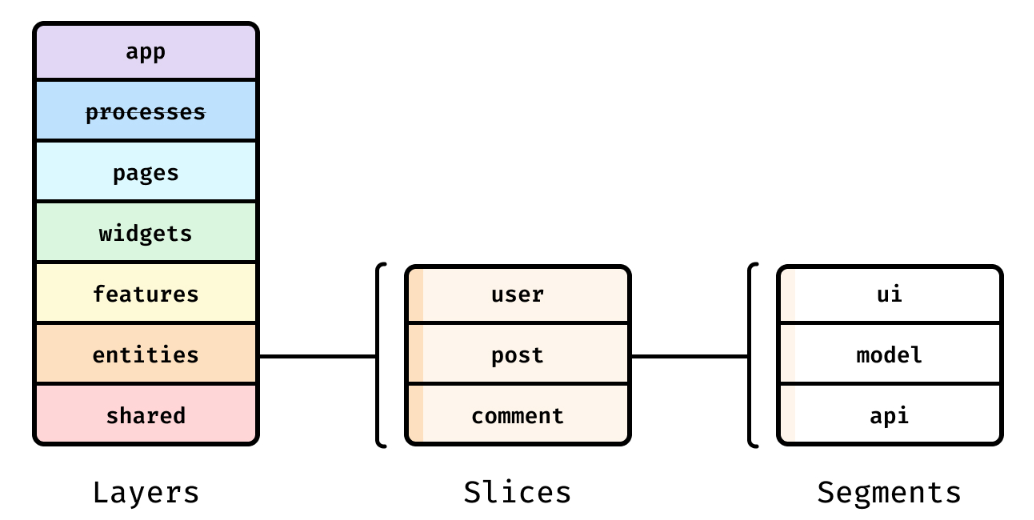
\includegraphics[scale=0.6]{styles/diploma/inc/fsd-pic1.png}
  \caption{Разделение проекта на слои, слайсы и сегменты}
  \label{fig:fsd}
\end{figure}

Данная методология обладает рядом преимуществ, которые делают его эффективным подходом для разработки фронтенд-проектов:

\begin{itemize}
    \item Архитектура FSD сосредоточена на бизнес-функциональности и разделяет код по функциональным возможностям. Это позволяет лучше структурировать и организовать код, делая бизнес-логику явной и понятной для разработчиков.
    \item Методология обеспечивает гибкость и адаптивность архитектуры. Компоненты могут быть легко заменены или добавлены в соответствии с новыми требованиями или условиями проекта. Это позволяет проекту быть более масштабируемым и способствует более простому внесению изменений.
    \item Архитектура FSD состоит из доменных модулей, таких как слои, слайсы и сегменты, что делает ее относительно простой для изучения и понимания. Разработчики могут быстро ориентироваться в структуре проекта и находить нужные модули, что способствует более эффективному сотрудничеству в команде.
    \item Благодаря структурированному подходу FSD, каждый модуль может быть независимо модифицирован или переписан без сайд-эффектов на другие модули. Это помогает управлять техническим долгом проекта и делает его более гибким для будущих изменений и развития.
    \item FSD находит баланс между принципом "Don't Repeat Yourself" (DRY) и локальной кастомизацией. Архитектура позволяет переиспользовать компоненты и модули, сохраняя при этом возможность их локальной настройки и кастомизации для конкретных потребностей проекта.
\end{itemize}

\subsubsection{Применение выбранной методологии в разработке}

Разработка по данной методологии начинается с определения и организации слоев. Каждый слой представляет собой логическую группировку модулей с определенными функциональными обязанностями. Слои включают shared, entities, features, widgets, pages, processes и app.

Рассмотрим алгоритм декомпозиции проекта на указанные слои по зонам ответственности. Когда разрабатывается новый модуль, разработчику необходимо определить к какому слою он должен относится. Представленные вопросы помогают отнести нужный модуль к нужному слою:

\begin{itemize}
    \item Shared: Это не относится к Бизнес-Логике и является общим переиспользуемым служебным кодом?
    \item Entities: Это относится непосредственно к бизнес-сущности?
    \item Features: Это относится к действию пользователя, представляющему бизнес-ценность?
    \item Widgets: Это самостоятельный и полноценный блок страницы с конкрытными действиями?
    \item Pages: Это относится к конкретной странице/экрану?
    \item Processes: Это относится к конкретному юзкейсу, протекающему через несколько страниц?
    \item App: Это общая инициализирующая логика приложения?
\end{itemize}

Рассмотрим каждый слой, отнеся к нему какой-нибудь модуль:

Shared: здесь располагаются переиспользуемые компоненты, например: кнопки, тексты, иконки, спиннеры, настройки безопасности, инстансы Axios, хуки, хелперы для работы со Store и т.д. Иными словами, компоненты без привязки к бизнес-логике. Пример представлен на рисунке~\ref{fig:fsd-shared}

\begin{figure}
  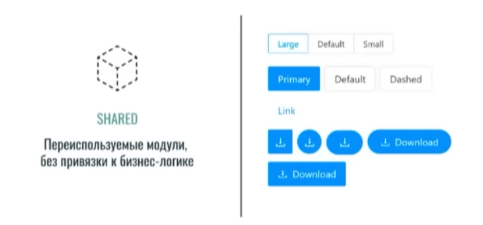
\includegraphics[scale=1]{styles/diploma/inc/fsd-shared.png}
  \caption{Слой Shared}
  \label{fig:fsd-shared}
\end{figure}

Entities: например карточка поста в соц-сети, на которой представленны только общие части, специфичные для всех постов. Функциональностей по типу лайков, вспомогательных кнопок, кнопки поделится и т.д., здесь не представлены. Они представлены в виде слотов, куда функциональности добавляются уже на уровне выше. Пример представлен на рисунке~\ref{fig:fsd-entities}

\begin{figure}
  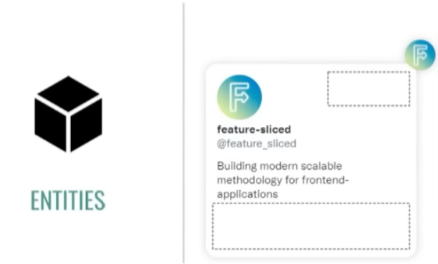
\includegraphics[scale=1]{styles/diploma/inc/fsd-entities.png}
  \caption{Слой Entities}
  \label{fig:fsd-entities}
\end{figure}

Features: здесь уже появляются функциональности, которые несут в себе какой-то бизнес-функционал, который приводит к какому-то результату, например: лайки, кнопка подписаться и т.д. Причем одна фича должна решать одну задачу. Пример представлен на рисунке~\ref{fig:fsd-features}

\begin{figure}
  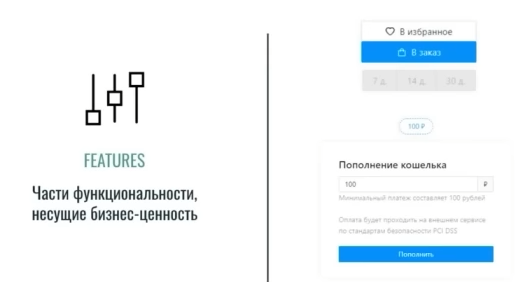
\includegraphics[scale=1]{styles/diploma/inc/fsd-features.png}
  \caption{Слой Features}
  \label{fig:fsd-features}
\end{figure}

Widgets: это комбинация entities, которые содержат "пустые слоты" и в эти слоты подставляются необходимые фичи (features). В данном случае, виджеты - это самостоятельные смысловые блоки, комбинирующие нижние слои. Полноценный пост, который можно оставить в группе - это уже виджет, причем один виджет может называть userPost, а другой groupPost, потому что с точки зрения функционала и работы с Backend они скорее всего будут разными. Пример представлен на рисунке~\ref{fig:fsd-widgets}

\begin{figure}
  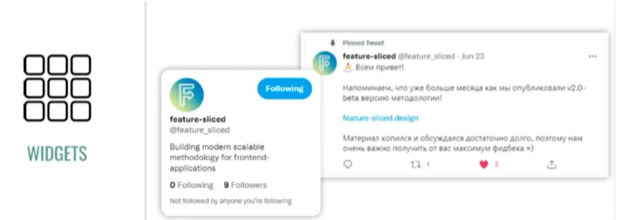
\includegraphics[scale=1]{styles/diploma/inc/fsd-widgets.png}
  \caption{Слой Widgets}
  \label{fig:fsd-widgets}
\end{figure}

Pages: страница собирается непосредственно из виджетов. Непосредственно в данном слои находится минимум бизнес-логики, запросов и прочего, все необходимое выносится на слои ниже. Пример представлен на рисунке~\ref{fig:fsd-pages}

\begin{figure}
  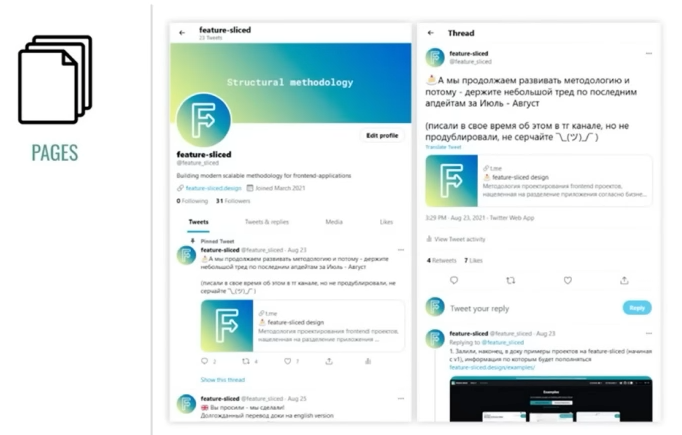
\includegraphics[scale=0.8]{styles/diploma/inc/fsd-pages.png}
  \caption{Слой Pages}
  \label{fig:fsd-pages}
\end{figure}

Processes: в нем хранится какой-то сложный набор действий, который протекает через несколько страниц. Например авторизация в несколько страниц.

App: данный слой хранит в себе инициализирующую логику приложения (Инициализирующая точка входа в приложение). Здесь хранятся все роутинг, провайдеры, глобальные стили, глобальные типы и все что не будет никогда и ни при каких условиях использоваться где-то ниже
